% Musterblatt Terme 4 (aus Muster 3: Kopf/Fuß, „Abschluss“, Schlusstest,
% a) vorgerechnet nur, wo es den Weg zeigt) – Ziel für das Skript
% Sechs Einheiten: 1 Zusammenfassen, 2 Malnehmen, 3 Klammern auflösen,
% 4 Ausklammern, 5 Termwerte, 6 Terme aufstellen; Blatt 0 davor.
% Je Verfahren eine Nummer (Leiter leicht → schwer). a) grau vorgerechnet
% nur in 14 (Ausklammern), den drei Klammer-Nummern und den Termwerten;
% sonst zeigt der Merkkasten das Beispiel. Marken klein rechts: „P10 ’jj“
% am Prüfungsoriginal, „GYM“ an dem, was nur das Gymnasium verlangt.
% „Abschluss“ (drei Teilaufgaben, mittlere Höhe) nur in Einheiten mit mehr
% als einem Verfahren (1, 2, 3, 6). Am Ende „Zum Schluss“: je Einheit eine
% Teilaufgabe, gemischt, dazu zwei höhere; Lösungen mit „falsch → Nr. n“.
% Quelle je Teilaufgabe im Kommentar davor: % <id> = wortgleich aus der
% Bank (Auftrag im Titel der Nummer), % GEÄNDERT <id> = Zahlen oder Form
% geändert, % NEU = nicht in der Bank. % pruef: … = Rechenprobe (pruef.py).
\documentclass[11pt]{article}
\usepackage{mathblatt}
\usepackage{multicol}
\usepackage{lastpage}
% Kopf: „Terme“ links; Fuß: Kennung klein links, „Seite n von m“ Mitte
\pagestyle{fancy}\fancyhf{}\renewcommand{\headrulewidth}{0pt}
\setlength{\headheight}{14pt}
\fancyhead[L]{\small Terme}
\fancyfoot[L]{\footnotesize\color{mbgrau}Muster 4 2026-10-01}
\fancyfoot[C]{\small Seite \thepage\ von \pageref{LastPage}}
\raggedright
\makeatletter
% ---------------------------------------------------------------- Satz
\newcommand{\vorgerechnet}[1]{\textcolor{gray!70}{#1}}
\newcommand{\einheit}[2]{\par\Needspace*{0.33\textheight}\addvspace{16pt}%
  \noindent{\Large\bfseries\ifblank{#1}{}{#1\hspace{0.6em}}#2}\par\nobreak\vspace{2pt}%
  \gappto\mblsg{\lsgeinheit{\ifblank{#1}{}{#1\ }#2}}}
% Hauptnummer; ohne Option bleibt sie auf einer Seite, mit [b] darf sie
% zwischen zwei Zeilen umbrechen (mindestens drei Zeilen je Seite)
\newsavebox{\nrbox}\newlength{\nrhoehe}
\newcommand{\nrtitel}[1]{\noindent\hangindent1.6em\hangafter1%
  \makebox[1.6em][l]{\textbf{\theaufgabe.}}#1\par\vspace{1pt}}
\newenvironment{nr}[2][]{\refstepcounter{aufgabe}\setcounter{teil}{0}%
  \def\nrart{#1}%
  \ifx\nrart\@empty
    \begin{lrbox}{\nrbox}\begin{minipage}[t]{\linewidth}\raggedright
    \setlength{\parskip}{0pt}\nrtitel{#2}%
  \else
    \par\addvspace{11pt}\Needspace*{8\baselineskip}\nrtitel{#2}%
  \fi}%
 {\ifx\nrart\@empty
    \end{minipage}\end{lrbox}%
    \setlength{\nrhoehe}{\dimexpr\ht\nrbox+\dp\nrbox\relax}%
    \par\addvspace{11pt}\Needspace*{\nrhoehe}\noindent\usebox{\nrbox}\par
  \else\par\fi}
\newcommand{\teilmarke}{\stepcounter{teil}\makebox[1.6em][r]{\alph{teil})\hspace{0.35em}}}
\newcommand{\marke}[1]{\ifblank{#1}{}{\hfill{\footnotesize #1}}}
\newlength{\feldbreite}\setlength{\feldbreite}{4.5cm}
\newcommand{\antwort}{\underline{\hspace{\feldbreite}}}
\newcommand{\zeilenluft}{\par\nobreak\vskip 12pt plus 1pt\relax}
\newcommand{\zeilenluftb}{\par\vskip 12pt plus 1pt\relax}
% Leiter: Zeilen gesammelt, am Ende gesetzt; Term linksbündig in einer
% Spalte so breit wie der breiteste Term, dann „=“ und Feld in fester
% Spalte; Umbruch nur mit mindestens drei Zeilen je Seite
\newlength{\kw}\newlength{\kwmax}
\newcounter{kzahl}\newcounter{kzeile}
\newcommand{\kliste}{}
\newcommand{\kmerke}[2]{\settowidth{\kw}{#1}%
  \ifdim\kw>\kwmax\global\kwmax=\kw\fi\stepcounter{kzahl}\gappto\kliste{#2}}
\newcommand{\kstart}[1]{\global\kwmax=0pt\setcounter{kzahl}{0}\setcounter{kzeile}{0}%
  \gdef\kliste{}\setlength{\feldbreite}{#1}}
\newcommand{\kende}{\par\vspace{3pt}\kliste\par}
\newcommand{\kettezeile}[1]{\stepcounter{kzeile}%
  \ifnum\value{kzeile}>1
    \ifnum\value{kzeile}<4 \zeilenluft
    \else\ifnum\numexpr\value{kzahl}-\value{kzeile}\relax<2 \zeilenluft
    \else\zeilenluftb\fi\fi
  \fi
  \noindent#1\par}
\newenvironment{kette}[1][4.5cm]{\kstart{#1}}{\kende}
\newcommand{\termspalte}[1]{\makebox[\kwmax][l]{$#1 =$}\hspace{0.6em}}
\NewDocumentCommand{\rk}{O{} m m}{\kmerke{$#2 =$}{\kettezeile{\teilmarke\lsgm{#3}%
  \termspalte{#2}\antwort\marke{#1}}}}
% vorgerechnet: nach „=“ grau Zwischenschritt und Ergebnis
\newcommand{\rkv}[2]{\kmerke{$#1 =$}{\kettezeile{\teilmarke\termspalte{#1}%
  \vorgerechnet{$#2$}}}}
% Termwert: Term, Einsetzung, Feld
\newenvironment{werte}[1][2.8cm]{\kstart{#1}}{\kende}
\newcommand{\wertkopf}[2]{$#1$\hspace{0.8em}für $#2$:}
\NewDocumentCommand{\rw}{O{} m m m}{\kmerke{\wertkopf{#2}{#3}}{\kettezeile{\teilmarke\lsgm{#4}%
  \makebox[\kwmax][l]{\wertkopf{#2}{#3}}\hspace{0.6em}\antwort\marke{#1}}}}
\newcommand{\rwv}[3]{\kmerke{\wertkopf{#1}{#2}}{\kettezeile{\teilmarke
  \makebox[\kwmax][l]{\wertkopf{#1}{#2}}\hspace{0.6em}\vorgerechnet{$#3$}}}}
% Unterstreichen
\newenvironment{liste}{\kstart{0pt}}{\kende}
\newcommand{\ru}[2]{\kmerke{}{\kettezeile{\teilmarke\lsgt{#2}#1}}}
\newcommand{\ruv}[1]{\kmerke{}{\kettezeile{\teilmarke#1}}}
\newcommand{\unter}[1]{{\color{gray!70}\underline{\color{black}#1}}}
% Textzeile, Feld direkt hinter dem Text
\NewDocumentCommand{\rt}{O{} m m}{\par\vspace{7pt}\noindent\hangindent1.6em\hangafter1
  \teilmarke\lsgt{#3}#2\nobreak\hspace{0.6em}\underline{\hspace{4cm}}\marke{#1}\par}
\newcommand{\rtv}[2]{\par\vspace{7pt}\noindent\hangindent1.6em\hangafter1
  \teilmarke#1\nobreak\hspace{0.6em}\vorgerechnet{#2}\par}
% Textzeile ohne Feld (Feld folgt neben der Figur)
\NewDocumentCommand{\rtx}{O{} m m}{\par\vspace{7pt}\noindent
  \ifblank{#1}{\parbox[t]{\linewidth}{\raggedright\hangindent1.6em\hangafter1
   \teilmarke\lsgt{#3}#2}}%
  {\parbox[t]{\dimexpr\linewidth-\kennbreite\relax}{\raggedright\hangindent1.6em\hangafter1
   \teilmarke\lsgt{#3}#2}\parbox[t]{\kennbreite}{\raggedleft\footnotesize #1}}\par}
% Textaufgabe mit Rechenraum, Marke klein rechts
\newlength{\kennbreite}\setlength{\kennbreite}{1.6cm}
\NewDocumentCommand{\rs}{O{} m m}{\par\vspace{9pt}\noindent
  \teilmarke\lsgt{#3}%
  \ifblank{#1}{\parbox[t]{\dimexpr\linewidth-1.6em\relax}{\raggedright #2}}%
   {\parbox[t]{\dimexpr\linewidth-1.6em-\kennbreite\relax}{\raggedright #2}%
    \parbox[t]{\kennbreite}{\raggedleft\footnotesize #1}}\par\raum}
\newcommand{\raum}{\par\nobreak\vspace{7mm}\noindent\hspace*{1.6em}%
  \rule{0.5\textwidth}{0.4pt}\par\nobreak\vspace{7mm}\noindent\hspace*{1.6em}%
  \rule{0.5\textwidth}{0.4pt}\par}
\newcommand{\kreuzzeile}[1]{\par\vspace{6pt}\noindent\hspace*{1.6em}#1\par}
\renewcommand{\kreuz}[1]{$\square$\,#1\hspace{2.2em}}
\newcommand{\figurfelder}[2]{\par\vspace{6pt}\noindent\hspace*{1.6em}%
  $\vcenter{\hbox{#1}}$\hspace{1.5em}\begin{tabular}[c]{@{}l@{\hspace{0.5em}}l@{}}#2\end{tabular}\par}
% Merkkasten: schmaler Rahmen über die Textbreite, keine Fläche, höchstens
% drei Zeilen (Regel, Musterterm, häufiger Fehler); hängt am Einheitentitel
\newcommand{\merk}[1]{\par\nobreak\vspace{5pt}\noindent
  \fcolorbox{black!60}{white}{\parbox{\dimexpr\linewidth-2\fboxsep-2\fboxrule\relax}{%
  \raggedright\setlength{\parskip}{1.5pt}#1}}\par\vspace{2pt}}
% ---------------------------------------------------------------- Lösungen
\newcommand{\mblsg}{}
\newcommand{\lsgm}[1]{\lsgt{$#1$}}
\newcommand{\lsgextra}{}
\newcommand{\lsgt}[1]{\xappto\mblsg{\noexpand\lz{\theaufgabe}{\alph{teil}}}%
  \xappto\mblsg{{\unexpanded{#1}\unexpanded\expandafter{\lsgextra}}}%
  \gdef\lsgextra{}}
% Zum Schluss: Zusatz zur nächsten Lösung; \falsch vor \rt/\rs,
% \falschk in kette/werte (wird mit der Zeile gesetzt)
\newcommand{\falsch}[1]{\gdef\lsgextra{\quad{\footnotesize falsch $\rightarrow$ Nr.~#1}}}
\newcommand{\falschk}[1]{\gappto\kliste{\falsch{#1}}}
\newcommand{\lzletzte}{0}
\newcommand{\lz}[3]{\par\noindent\hangindent3.4em\hangafter1
  \ifnum#1=\lzletzte\relax\makebox[1.8em][l]{}\else\makebox[1.8em][l]{\textbf{#1}}\fi
  \gdef\lzletzte{#1}%
  \makebox[1.6em][l]{\ifx&#2&\else#2)\fi}#3\par}
\newcommand{\lsgeinheit}[1]{\par\addvspace{4pt}\noindent{\bfseries #1}\par}
\makeatother

\begin{document}
\setlength{\parskip}{0pt}

% =================================================================== Blatt 0
\einheit{}{Das kennst du schon}
\noindent
\begin{minipage}[t]{0.48\linewidth}
\begin{nr}{Plus und Minus}
\begin{kette}[2cm]
% terme-zone-f1-v1
\rk{4 - 9}{-5}
% terme-zone-f1-v4
\rk{-6 - 4}{-10}
% terme-zone-f1-v3
\rk{-2{,}5 + 1}{-1{,}5}
% NEU
\rk{-1{,}5 - (-4)}{2{,}5}
\end{kette}
\end{nr}
\begin{nr}{Mal mit Vorzeichen}
\begin{kette}[2cm]
% terme-zone-f2-v1
\rk{(-5) \cdot 2}{-10}
% terme-zone-f2-v4
\rk{(-4) \cdot (-5)}{20}
% terme-zone-f2-v3
\rk{(-0{,}5) \cdot 8}{-4}
% NEU
\rk{(-1{,}5) \cdot (-4)}{6}
\end{kette}
\end{nr}
\end{minipage}\hfill
\begin{minipage}[t]{0.48\linewidth}
\begin{nr}{Dezimalzahlen und Brüche}
\begin{kette}[2cm]
% terme-zone-f3-v4
\rk{0{,}9 + 0{,}3}{1{,}2}
% terme-zone-f3-v3
\rk{0{,}5 - 1{,}5}{-1}
% terme-zone-f3-v2
\rk{\frac{1}{2} + \frac{1}{4}}{\frac{3}{4}}
% NEU
\rk{-0{,}4 - 0{,}8}{-1{,}2}
\end{kette}
\end{nr}
\begin{nr}{Punkt vor Strich}
\begin{kette}[2cm]
% terme-zone-f4-v1
\rk{5 + 2 \cdot 4}{13}
% terme-zone-f4-v3
\rk{6 - 4 \cdot 2{,}5}{-4}
% NEU
\rk{2 - 3 \cdot (-4)}{14}
\end{kette}
\end{nr}
\end{minipage}

% =================================================================== Einheit 1
\einheit{1}{Terme zusammenfassen}
\merk{Nur gleiche Variablen mit gleicher Hochzahl zusammenfassen: Vorzahlen addieren, die Variable bleibt.\par
$3x + 5x = 8x$ \qquad $7a - 2a + 4 = 5a + 4$ \qquad $x^2 + 3x$ bleibt so\par
Achtung: $3x + 4 \neq 7x$ \qquad $x + 6x = 7x$, nicht $6x$}

\begin{nr}{Gleichartige Glieder erkennen – unterstreiche, was zusammengehört.}
\begin{liste}
% terme-e2-k1-s0-v1
\ru{$4y$, \quad $7$, \quad $9y$}{$4y$ und $9y$}
% terme-e2-k1-s0-v3
\ru{$5x^2$, \quad $4x$, \quad $3x^2$}{$5x^2$ und $3x^2$}
% NEU
\ru{$3ab$, \quad $2a$, \quad $-ab$, \quad $5b$}{$3ab$ und $-ab$}
% NEU
\ru{$2x^2y$, \quad $3xy^2$, \quad $-x^2y$, \quad $4xy$, \quad $-xy^2$}{$2x^2y$ und $-x^2y$; $3xy^2$ und $-xy^2$}
\end{liste}
\end{nr}

\begin{nr}[b]{Terme zusammenfassen}\label{nr:zus}
\begin{kette}
% terme-e2-k4-s1-v1
\rk{7x + 2x}{9x}
% terme-e2-k4-s2-v3
\rk{13b - 7b}{6b}
% terme-e2-k4-s3-v3
\rk{10b - 3b - 4b}{3b}
% terme-e2-k4-s4-v3
\rk{10 + 6x - 2x}{4x + 10}
% terme-e2-k4-s5-v3
\rk{3b + 6a + 5b}{6a + 8b}
% NEU
\rk{-2x + 7 - x - 9}{-3x - 2}
% terme-e2-k4-s9-v2
\rk{3a + 2a^2 + 4a}{2a^2 + 7a}
% NEU
\rk{1{,}5x^2 - 2x + 0{,}5x - 3x^2 + 4}{-1{,}5x^2 - 1{,}5x + 4}
% NEU
\rk[GYM]{\frac{1}{2}a + 3ab - \frac{3}{4}a - 5ab + 2b}{-\frac{1}{4}a - 2ab + 2b}
\end{kette}
\end{nr}

\begin{nr}{Abschluss – fasse zusammen.}
\begin{kette}
% NEU
\rk{4x - 3y + 2 - x + 5y}{3x + 2y + 2}
% NEU
\rk{2{,}5a^2 + a - a^2 - 3{,}5a}{1{,}5a^2 - 2{,}5a}
\end{kette}
% terme-e2-k6-s4-v2
% pruef: s + 2*s + s + 2*s == 6*s
% pruef: 6*8 == 48
\rs{Ein Beet ist $s$ Meter breit und doppelt so lang. Um das Beet kommt ein Zaun. Stelle einen Term für die Länge des Zauns auf und fasse ihn zusammen. Wie viele Meter Zaun braucht man bei $s = 8$?}{$6s$; 48 m}
\end{nr}

% =================================================================== Einheit 2
\einheit{2}{Terme malnehmen}
\merk{Zahlen mal Zahlen, Variablen mal Variablen.\par
$3 \cdot 4x = 12x$ \qquad $2x \cdot 3x = 6x^2$ \qquad $3a \cdot 2b = 6ab$\par
Achtung: $x \cdot x = x^2$, nicht $2x$}

\begin{nr}[b]{Terme malnehmen}\label{nr:mal}
\begin{kette}
% terme-e2-k5-s1-v1
\rk{5 \cdot 2x}{10x}
% terme-e2-k5-s2-v2
\rk{7b \cdot 4}{28b}
% terme-e2-k5-s3-v1
\rk{4y \cdot 2y}{8y^2}
% terme-e2-k5-s4-v2
\rk{3 \cdot (-6a)}{-18a}
% terme-e2-k5-s5-v2
\rk{2x \cdot 7y}{14xy}
% terme-e2-k5-s7-v2
\rk{(-4x) \cdot 3y \cdot (-2)}{24xy}
% NEU
\rk{(-2a) \cdot 3ab \cdot (-a)}{6a^3b}
% NEU
\rk{-\frac{2}{3}x \cdot 6y \cdot (-xy)}{4x^2y^2}
% NEU
\rk[GYM]{3x \cdot 2y - 4xy + x \cdot (-5y) + 2y \cdot 3x}{3xy}
% NEU
\rk[GYM]{2a \cdot 3a - a \cdot (-4a) + 5a^2 \cdot 2 - 3 \cdot 7a^2}{-a^2}
\end{kette}
\end{nr}

\begin{nr}{Abschluss – vereinfache.}
\begin{kette}
% NEU
\rk{4x \cdot 3 - 5x}{7x}
% NEU
\rk{-y \cdot 4y + 3y^2 - y}{-y^2 - y}
\end{kette}
% NEU
% pruef: 2*x*3*x*5 == 30*x**2
\rt{Ein Quader hat die Kantenlängen $2x$, $3x$ und $5$ (in cm). Gib einen Term für das Volumen an und vereinfache.}{$30x^2$}
\end{nr}

% =================================================================== Einheit 3
\einheit{3}{Klammern auflösen}
\merk{Plus vor der Klammer: Klammer weglassen. \hfill $a + (b - c) = a + b - c$\par
Minus vor der Klammer: alle Vorzeichen drehen. \hfill $a - (b - c) = a - b + c$ \quad Achtung: $-(x - 4) = -x + 4$\par
Zahl mal Klammer: jedes Glied malnehmen. \hfill $3 \cdot (x + 4) = 3x + 12$}

\begin{nr}[b]{Plusklammer und Minusklammer – löse auf und fasse zusammen, wo es geht.}\label{nr:pm}
\begin{kette}
% terme-e3-k2-s1-v1 (vorgerechnet)
\rkv{5a + (2b - 1)}{5a + 2b - 1}
% terme-e3-k2-s4-v1
\rk{5a - (2b + 4)}{5a - 2b - 4}
% terme-e3-k2-s4-v2
\rk{8x - (3y - 6)}{8x - 3y + 6}
% terme-e3-k2-s5-v1
\rk{7a - (2b - 5 + c)}{7a - 2b + 5 - c}
% terme-e3-k2-s5-v3
\rk{10 - (3a - 4b + 6c)}{10 - 3a + 4b - 6c}
% NEU
\rk{4{,}5 - (-x + 2{,}5y - 1{,}5)}{x - 2{,}5y + 6}
% NEU
\rk{-(a^2 - 2ab) + (3ab - a^2) - (-b^2)}{-2a^2 + 5ab + b^2}
\end{kette}
\end{nr}

\begin{nr}[b]{Mal Klammer – löse die Klammer auf.}
\begin{kette}
% GEÄNDERT terme-e3-k2-s2-v1 (Form: ohne Tabelle; vorgerechnet)
\rkv{5 \cdot (x + 3)}{5 \cdot x + 5 \cdot 3 = 5x + 15}
% GEÄNDERT terme-e3-k2-s2-v2 (Form: ohne Tabelle)
\rk{4 \cdot (a + 7)}{4a + 28}
% terme-e3-k2-s6-v1
\rk{-2 \cdot (x + 5)}{-2x - 10}
% terme-e3-k2-s6-v2
\rk{-3 \cdot (a - 7)}{-3a + 21}
% NEU
\rk{2x \cdot (3x - 4)}{6x^2 - 8x}
% NEU
\rk{(a - 2b + 5) \cdot (-4)}{-4a + 8b - 20}
% NEU
\rk{-0{,}5y \cdot (4y - 6 + 2x)}{-2y^2 + 3y - xy}
% NEU
\rk{\frac{2}{3}a \cdot (9ab - 6a + 3)}{6a^2b - 4a^2 + 2a}
\end{kette}
\end{nr}

\begin{nr}[b]{Klammern auflösen und zusammenfassen}\label{nr:kz}
\begin{kette}
% terme-e3-k2-s7-v1 (vorgerechnet)
\rkv{5x + 2 \cdot (x + 6)}{5x + 2x + 12 = 7x + 12}
% terme-e3-k2-s7-v2
\rk{9a - (4a + 3)}{5a - 3}
% terme-e3-k2-s7-v3
\rk{6 + 4 \cdot (y - 1)}{4y + 2}
% terme-e3-k2-s8-v1
\rk{3 \cdot (2x + 5) - 2 \cdot (x - 4)}{4x + 23}
% terme-e3-k2-s8-v3
\rk{-3 \cdot (b - 2) + 7 \cdot (b + 1)}{4b + 13}
% NEU
\rk{2a \cdot (a - 3) - a \cdot (5 - a)}{3a^2 - 11a}
% NEU
\rk{5x - [\,2 - 3 \cdot (x - 4)\,]}{8x - 14}
% NEU
\rk[GYM]{3x - \{\,2y - [\,x - (y - 4x)\,]\,\}}{8x - 3y}
% NEU
\rk[GYM]{-2a \cdot (3b - a) + 3 \cdot (ab - 2a^2) - a \cdot (-b)}{-4a^2 - 2ab}
% NEU
\rk[GYM]{\frac{1}{2} \cdot (6x - 4y) - \frac{3}{4} \cdot (8y - 4x)}{6x - 8y}
\end{kette}
\end{nr}

\begin{nr}{Abschluss – vereinfache.}
\begin{kette}
% NEU
\rk{7y - (2y - 3) + 2 \cdot 4y}{13y + 3}
% NEU
\rk{x \cdot (x + 3) - x^2}{3x}
\end{kette}
% terme-e3-k3-s4-v1
% pruef: 9*(24 + x) == 216 + 9*x
\rs{Ein Kinoticket kostet 9 €. Eine Klasse mit 24 Schülern nimmt noch $x$ Begleiter mit. Schreibe die Gesamtkosten in Euro als Term mit Klammer. Löse die Klammer auf.}{$9 \cdot (24 + x) = 216 + 9x$}
\end{nr}

% =================================================================== Einheit 4
\einheit{4}{Ausklammern}
\merk{Gemeinsamen Faktor vor die Klammer; Probe durch Ausmultiplizieren.\par
$6x + 9 = 3 \cdot (2x + 3)$ \qquad $4a^2 + 2a = 2a \cdot (2a + 1)$\par
Achtung: $8x - 8 = 8 \cdot (x - 1)$, die 1 bleibt in der Klammer}

\begin{nr}[b]{Ausklammern – klammere so viel aus wie möglich.}\label{nr:aus}
\begin{kette}
% terme-e4-k2-s1-v1 (vorgerechnet)
\rkv{5x + 10}{5 \cdot x + 5 \cdot 2 = 5 \cdot (x + 2)}
% terme-e4-k2-s1-v2
\rk{5x + 25}{5 \cdot (x + 5)}
% terme-e4-k2-s2-v1
\rk{x^2 + 5x}{x \cdot (x + 5)}
% terme-e4-k2-s3-v2
\rk{8a^2 - 20a}{4a \cdot (2a - 5)}
% terme-e4-k2-s4-v3
\rk{9y^2 + 9y}{9y \cdot (y + 1)}
% terme-e4-k2-s5-v2
\rk{5a^2 - 10a + 15}{5 \cdot (a^2 - 2a + 3)}
% terme-e4-k2-s10-v2
\rk{5x^2 + 10xy - 15x}{5x \cdot (x + 2y - 3)}
% NEU
\rk{-6a^2b + 9ab^2 - 3ab}{-3ab \cdot (2a - 3b + 1)}
% NEU
\rk{1{,}5x^3 - 4{,}5x^2 + 0{,}5x}{0{,}5x \cdot (3x^2 - 9x + 1)}
% NEU
\rk[GYM]{4x \cdot (a + b) - 3y \cdot (a + b)}{(a + b) \cdot (4x - 3y)}
% NEU
\rk[GYM]{\frac{3}{4}x^2y - \frac{1}{4}xy^2 + \frac{1}{2}xy}{\frac{1}{4}xy \cdot (3x - y + 2)}
\end{kette}
% NEU
% pruef: 2*a*a + 2*a*5 == 2*a*(a + 5)
\rtx[GYM]{Zwei Rechtecke liegen nebeneinander. Gib den Flächeninhalt der ganzen Figur als Summe der Teilflächen und als Produkt mit Klammer an.}{$2a^2 + 10a = 2a \cdot (a + 5)$}
\figurfelder{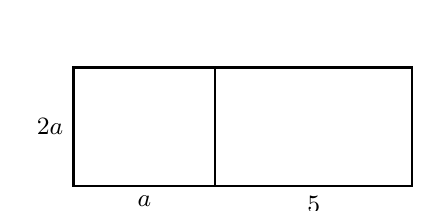
\begin{tikzpicture}[line width=0.8pt]
\draw (0,0) rectangle (1.8,1.5); \draw (1.8,0) rectangle (4.3,1.5);
\node[left,font=\small] at (0,0.75) {$2a$};
\node[below,font=\small] at (0.9,0) {$a$};
\node[below,font=\small] at (3.05,0) {$5$};
\end{tikzpicture}}{Summe: & \underline{\hspace{4.5cm}} \\[8mm]
Produkt: & \underline{\hspace{4.5cm}}}
\end{nr}

% =================================================================== Einheit 5
\einheit{5}{Termwerte berechnen}
\merk{Negative Zahlen in Klammern einsetzen: \ $3x^2$ für $x = -2$: \ $3 \cdot (-2)^2 = 12$}

\begin{nr}[b]{Termwerte berechnen – setze ein und rechne.}\label{nr:wert}
\begin{werte}
% terme-e1-k2-s1-v1 (vorgerechnet)
\rwv{4x - 3}{x = 5}{4 \cdot 5 - 3 = 17}
% terme-e1-k2-s1-v2
\rw{2x + 9}{x = -3}{3}
% terme-e1-k2-s1-v3
\rw{10 - 3x}{x = -2}{16}
% NEU
\rw{x^2 - 4x}{x = -3}{21}
% NEU
\rw{3x^2 - 2x}{x = -\frac{1}{2}}{\frac{7}{4}}
% NEU
\rw{\frac{1}{2}a - 3b}{a = 6,\ b = -\frac{2}{3}}{5}
% NEU
\rw{2 \cdot (x - y)^2 - xy}{x = -1,\ y = 2}{20}
\end{werte}
% terme-e2-k4-s11-v1
% pruef: 8*3 - 2*3**2 - 5*3 == -9
\rs[P10 ’25]{Vereinfache den Term $8a - 2a^2 - 5a$ und berechne seinen Wert für $a = 3$.}{$3a - 2a^2$; für $a = 3$: $-9$}
\end{nr}

% =================================================================== Einheit 6
\einheit{6}{Terme aufstellen}
\merk{„um 5 vermindert“: \ $x - 5$ \qquad „das Doppelte der Summe aus $x$ und 5“: \ $2 \cdot (x + 5)$, mit Klammer}

\begin{nr}[b]{Terme aufstellen – schreibe einen Term.}\label{nr:auf}
% terme-e1-k1-s2-v2
% pruef: 2*x - 5 == 2*x - 5
\rt{Das Doppelte einer Zahl $x$ wird um 5 vermindert.}{$2x - 5$}
% terme-e1-k1-s4-v1
% pruef: 4*a + 3*b == 4*a + 3*b
\rt{Ein Heft kostet $a$ Euro, ein Stift $b$ Euro. Lena kauft 4 Hefte und 3 Stifte. Was zahlt sie?}{$4a + 3b$}
% GEÄNDERT terme-e1-k1-s3-v3 (Form: Feld neben der Figur)
% pruef: 2*x + 14 == x + 7 + x + 7
\rtx{Umfang des Rechtecks (Maße in cm):}{$2x + 14$}
\figurfelder{\rechteck[seiten={7,x,,},punkte=]{3.2}{1.1}}{& \underline{\hspace{4cm}}}
% terme-e1-k1-s6-v2
% pruef: 5*(4*x - 1) == 20*x - 5
\rt{Nimm das Vierfache einer Zahl $x$, subtrahiere 1 und multipliziere die Differenz mit 5.}{$5 \cdot (4x - 1)$}
% NEU
% pruef: 3*(x + x - 3) == 6*x - 9
\rt[GYM]{Lea ist $x$ Jahre alt, ihr Bruder ist 3 Jahre jünger. Die Mutter ist dreimal so alt wie beide zusammen. Wie alt ist die Mutter?}{$3 \cdot (x + x - 3) = 6x - 9$}
% NEU
% pruef: 3*x*2 + x*x == 6*x + x**2
% pruef: 3*x + 2 + 2*x + x + x + (2 + x) == 8*x + 4
\rtx[GYM]{Die Figur besteht aus zwei Rechtecken (Maße in cm). Gib Terme für den Flächeninhalt und den Umfang an und fasse sie zusammen.}{Fläche: $x^2 + 6x$; Umfang: $8x + 4$}
\figurfelder{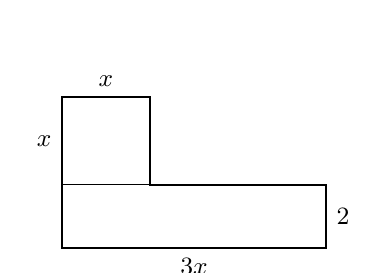
\begin{tikzpicture}[line width=0.8pt,scale=0.8]
\draw (0,0) -- (4.2,0) -- (4.2,1.0) -- (1.4,1.0) -- (1.4,2.4) -- (0,2.4) -- cycle;
\draw[line width=0.4pt] (0,1.0) -- (1.4,1.0);
\node[below,font=\small] at (2.1,0) {$3x$};
\node[right,font=\small] at (4.2,0.5) {$2$};
\node[above,font=\small] at (0.7,2.4) {$x$};
\node[left,font=\small] at (0,1.7) {$x$};
\end{tikzpicture}}{Flächeninhalt: & \underline{\hspace{4cm}} \\[8mm]
Umfang: & \underline{\hspace{4cm}}}
% terme-e1-k1-s7-v1
\rtx[P10 ’23]{Die Differenz aus dem Dreifachen einer Zahl $x$ und 7 wird verdoppelt. Kreuze den passenden Term an.}{$2 \cdot (3x - 7)$}
\kreuzzeile{\kreuz{$(3x - 7) : 2$}\kreuz{$3x : 7 \cdot 2$}\kreuz{$2 \cdot (3x - 7)$}\kreuz{$3x - 7 \cdot 2$}}
\end{nr}

\begin{nr}{Abschluss}
% NEU
% pruef: 3*(x + 4) == 3*x + 12
\rt{Schreibe als Term: das Dreifache der Summe aus einer Zahl $x$ und 4.}{$3 \cdot (x + 4)$}
% NEU
% pruef: 3*(5*x - 3) == 15*x - 9
\rt{Die Differenz aus dem Fünffachen einer Zahl $x$ und 3 wird verdreifacht.}{$3 \cdot (5x - 3)$}
% terme-e1-k4-s4-v2
% pruef: 4.5 + 2.5*9 == 27
\rs{Ein Taxi kostet 4,50 € Grundpreis und 2,50 € je Kilometer. Stelle einen Term für den Fahrpreis in Euro bei $d$ Kilometern auf. Reichen 25 € für eine Fahrt von 9 km?}{$4{,}50 + 2{,}50d$; nein, 27 €}
\end{nr}

% =================================================================== Zum Schluss
% Je Einheit eine Teilaufgabe mittlerer Höhe (a–f, gemischt), dann zwei
% höhere (g GYM wie 12 h, h P10 ’25 wie 15 h), neue Zahlen; ungeteilt.
\par\addvspace{10pt}
\begin{nr}{Zum Schluss}
\begin{werte}
% NEU (Einheit 5; aus „Gemischt“ von Muster 3)
\falschk{\ref{nr:wert}}
\rw{5 - 2x^2}{x = -1{,}5}{0{,}5}
\end{werte}
\begin{kette}
% NEU (Einheit 3)
\falschk{\ref{nr:kz}}
\rk{4 \cdot (2a - 3) - (5a - 7)}{3a - 5}
% NEU (Einheit 1)
\falschk{\ref{nr:zus}}
\rk{2x + 5y - 6x + y}{-4x + 6y}
\end{kette}
% NEU (Einheit 4; aus „Gemischt“ von Muster 3)
% pruef: 7*b*(2*a - 3) == 14*a*b - 21*b
\falsch{\ref{nr:aus}}
\rt{Klammere aus: \ $14ab - 21b$}{$7b \cdot (2a - 3)$}
\begin{kette}
% NEU (Einheit 2)
\falschk{\ref{nr:mal}}
\rk{3x \cdot (-2xy)}{-6x^2y}
\end{kette}
% NEU (Einheit 6)
% pruef: 12 + 6*x == 12 + 6*x
\falsch{\ref{nr:auf}}
\rt{Ein Fitnessstudio kostet 12 € Grundgebühr und 6 € je Besuch. Stelle einen Term für die Kosten in Euro bei $x$ Besuchen auf.}{$12 + 6x$}
\begin{kette}
% NEU (GYM, wie 12 h)
\falschk{\ref{nr:pm}, \ref{nr:kz}}
\rk[GYM]{2a - \{\,3b - [\,a - (2b - 3a)\,]\,\}}{6a - 5b}
\end{kette}
% GEÄNDERT terme-e2-k4-s11-v1 (Zahlen; wie 15 h)
% pruef: 6*b - 3*b**2 - 2*b == 4*b - 3*b**2
% pruef: 4*(-2) - 3*(-2)**2 == -20
\falsch{\ref{nr:zus}, \ref{nr:wert}}
\rs[P10 ’25]{Vereinfache den Term $6b - 3b^2 - 2b$ und berechne seinen Wert für $b = -2$.}{$4b - 3b^2$; für $b = -2$: $-20$}
\end{nr}

% =================================================================== Lösungen
\clearpage
\noindent{\Large\bfseries Lösungen}\par\vspace{2pt}
\begin{multicols}{2}\raggedright\small\linespread{0.96}\selectfont
\mblsg
\end{multicols}
\end{document}
